\documentclass{article}
\usepackage[utf8]{inputenc}
\usepackage[english]{babel}
\usepackage{mathtools}
\usepackage{graphicx}

\usepackage{multicol}
 
\addtolength{\oddsidemargin}{-1.5in}
\addtolength{\evensidemargin}{0in}
\addtolength{\textwidth}{3in}

\addtolength{\topmargin}{-1.475in}
\addtolength{\textheight}{1.75in} 
 
 
\begin{document}
\begin{multicols}{3}
[
\section{NE101 Mid Term 2}
NE101 Equation Sheet, Joshua Howland, 11/3/2014]

Constants:\\
$\mu_{0} = 4 \pi \times 10 ^{-7} NA^{-2}$ or $Hm^{-1} $\\
$\epsilon = 8.854187 \times 10 ^{-12} \frac{F}{m}$\\	
$eV = 1.6022\times 10 ^{-19} J$\\
mass hydrogen $ = 1.00794u  $\\
$1u = 1.66053 \times 10^{-27} kg $\\
fine structure constant: \\
$\frac{e^{2}}{4\pi\epsilon_{0}} = 1.439976 Mev \cdot fm$\\
Avagadros number: $6.02214\times 10^{23}$\\
Electron charge: $1.602176\times 10^{-19} C$\\
1 barn = $10^{-24} cm^{2}$\\
1 fm = $10^{-15}$m
Boltzmann Constant:\\
$k_{B} = 1.3806488\times 10^{-23}JK^{-1}$\\
$k_{B} = 8.6173324\times 10^{-5}eVK^{-1}$\\
Mass neutron $= 1.008664916 u$\\

Nuclear radius ($\approx$): $ R = 1.25A^{1/3} fm$\\

Radioactive Decay:\\
ADD STUFF HERE!\\
Specific Solutions:\\
$R = N_{0}\sigma I$\\
$dN_{1} = N_{1}\lambda + RRdt$\\
$N_{1}(t) = \frac{R}{\lambda_{1}}(1 - e^{-\lambda_{1}t})$\\


Shell model:\\
Intermediate Form: (unlikely on exam):\\
Magic Numbers: 2,8,20,40,58,92,112 \\

Intermediate form with spin orbit (Extreme independent shell model):\\
$1s_{1/2}^{2} 1p_{3/2}^{4} 1p_{1/2}^{2} 1d_{5/2}^{6} 2s_{1/2}^{2} 1d_{3/2}^{4} 1f_{7/2}^{8} 2p_{3/2}^{4} $\\
$1f_{5/2}^{6} 2p_{1/2}^{2} 1g_{9/2}^{10} 1g_{7/2}^{8} 2d_{5/2}^{6} 2d_{3/2}^{4}$\\
Magic Numbers: 2, 8, 20, 28, 50, 82, 126, 184\\
Notation: 1(s-0, p-1, d-2, f-3, g-4, h-5)\\

Even-Odd nuclei:\\
To calculate parity, find unpaired proton/neutron shell state.  $l$ is the shell (s p d f..) and I is the subscript.  Find parity from l.  For excited states, bump the unpaired neutron up the number of excited states.
\hspace*{0.01\textwidth} Example: Give the expected shell-model spin and parity assignments for the ground states of: (a) $ \prescript{7}{}{Li} $: 3p, 4n: 1 unpaired proton.  Proton shells are: $1s_{1/2}^{2}1p_{3/2}^{1}$.  $\ell = 1 (p=1)$, $\pi = -$, $J_{\pi} = \frac{3}{2}^{-}$ (b) $ \prescript{11}{}{B} $: 5p, 6n: 1 unpaired proton.  Proton shells are: $1s_{1/2}^{2}1p_{3/2}^{3}$.  $\ell = 1 (p=1)$, $\pi = -$, $J_{\pi} = \frac{3}{2}^{-}$ (c) $ \prescript{15}{}{B} $: 6p, 9n: 1 unpaired neutron.  Neutron shells are: $1s_{1/2}^{2}1p_{3/2}^{4}1p_{1/2}^{2}1d_{5/2}^{1}$.  $\ell = 2(d=2)$, $\pi = +$, $J_{\pi} = \frac{5}{2}^{+}$ Note: $\prescript{15}{}{C}$ prediction wrong, observed value is $\frac{1}{2}^{+}$\\
ADD EXCITATION EX!\\

For odd-odd nuclei: $\vec{I} = \vec{j}_{p} + \vec{j}_{n}$\\
In ground state, $\vec{s}_{p}$ and $\vec{s}_{n}$ are parallel\\
$j_{p} = \ell_{p} + s_{p}$ and $j_{n} = \ell_{n} + s_{n}$\\
Note: $\ell$ and $s$ not always parallel!\\
To calculate $J_{\pi}$, match $\ell$ to correct orbital for p and n, with spins parallel and multiply parities!\\
Ex: $\prescript{40}{19}{K}_{21}$.  $J\pi$ found by coupling J from upaired p and n.  P: $1d_{3/2}$, N $1f_{7/2}$.  Put spins parallel, combine, mult parities.  Answer: $2^{-}$


EVEN EVEN:\\
Shell model predicts that even-even nuclei will have a spin of $0^{+}$
For excited states (even-even), the SHELL model predicts that the ground state is $0^{+}$, the first excited state is $2^{+}$, second is $4^{+}$ and so on.\\

Unit of EM energy called photon.  "Quantum" of vibrational energy called phonon\\
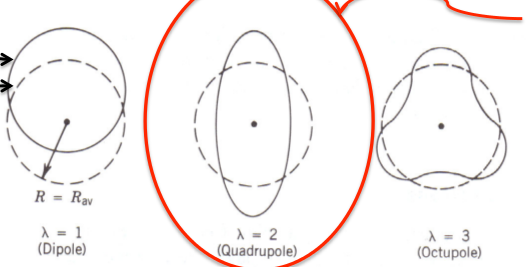
\includegraphics[width=4cm]{images/vibrations.jpg}\\
Energy of vibration: $E = hv$, v = frequency in $\frac{vibrations}{sec}$
Magnetic moments for first $2^{+}$ states predicted to be $2(\frac{Z}{A})$ and $\frac{E(4^{+})}{E(2^{+})}$ is predicted to $=2$ \\
Example:  Compute vibrational frequency associated with typical quadrupole vibrations, then compare typical lifetimes of $2^{+}$ excited states in vibrational nuclei to their vibrational frequency:  $\prescript{120}{}{Te}$ is a good choice (even-even, A<150), low lying excited state at $2^{+}$.  $E = hv$, $v = \frac{E}{h} = \frac{0.5604Mev}{4.135\times10^{-21}\frac{Mev}{s}} = 1.355\times10^{20}\frac{1}{sec}$.  T is much shorter than half life, so vibrates many times before decaying. $<\alpha>$ goes to 0, so we cant observe anything based on it, however $<\alpha^{2}>$ does not!

Nuclear Rotations:  Can only be observed in nuclei with non-spherical equilibrium shapes\\
$R(\theta,\phi) = R_{av}[1+\beta Y_{20}(\theta,\phi)]$\\
$\beta = \frac{4}{3} \sqrt{\frac{\pi}{5}} \frac{\Delta R}{R_{av}}$, $R_{av} = R_{0}A^{\frac{1}{3}}$\\
$E = \frac{\hbar^{2}}{2\Im}J(J+1)$, $\Im$= moment of inertia\\
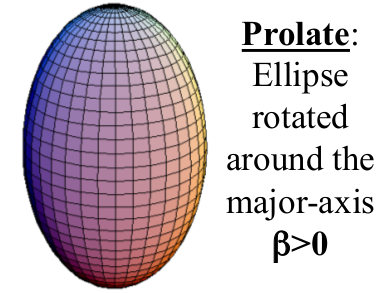
\includegraphics[width=3cm]{images/prolate.png}
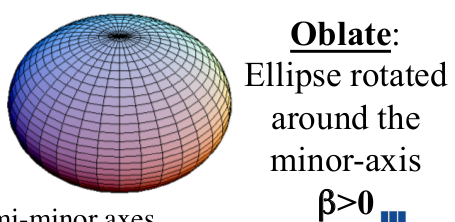
\includegraphics[width=3cm]{images/oblate.png}\\
$P = \frac{N_{p}^{valence}N_{n}^{valence}}{N_{p}^{valence}+N_{n}^{valence}}$, $P>4$ deformed\\
If the nucleus was rigid: $\Im_{rigid} = \frac{2}{5}MR_{av}^{2}(1+0.31\beta) \approx 6 kev$ for A = 170, but the observed value is 15Kev, so rotation is non rigid.  $\omega_{rotation} \approx 10^{20} \frac{rad}{sec} \approx 0.002c$ on surface.  Nuclear rotation is much slower than motion of nucleons, thus it is a type of collective motion. Deformation lowers energies of states moving inside the nucleus, raises energies of states spending more time outside nucleus\\??Add backbending/nisson model??\\
Collective model magnetic moment: 
$\mu (I) = I \frac{Z}{A} \mu_{N}$\\

Alpha Decay: First type of decay discovered, least penetrating, emitted almost entirely by large nuclei, p conserved\\
 $(Z,A)\rightarrow(Z-2,A-4) + \prescript{4}{2}{He}_{2}$\\
 $Q_{\alpha} = M(Z,A)c^{2} - M_{product}c^{2} - M(\prescript{4}{2}{He}_{2})$\\
 $Q_{\alpha} = K.E.(Z-2,A-4) + K.E.(\prescript{4}{2}{He}_{2})$\\
 $K.E. = T = \frac{p^{2}}{2m}$\\
 $Q = T_{\alpha} + T_{Z-2,A-4} = T_{\alpha} + \frac{p^2}{2M_{Z-2,A-4}}$\\
 $Q = T_{\alpha} + T_{\alpha}(\frac{M_{\alpha}}{M_{Z-2,A-4}})$\\
 $T_{\alpha} = \frac{Q}{1 + \frac{M_{\alpha}}{M_{Z-2,A-4}}} = \frac{Q}{1 + \frac{4}{A}}$\\
 $T_{x^{\prime}} = \frac{Q}{1 + \frac{m_{x^{\prime}}}{m_{\alpha}}}$\\
Example: $Q_{\alpha} = [M(\prescript{235}{}{U}) - M(\prescript{231}{}{Th}) - M(\alpha)]c^{2} = 4.678 Mev$.  $T_{\alpha} = 4.678Mev(1-\frac{4}{235}) = 4.598 Mev$, $T_{\prescript{231}{}{Th}} = Q_{\alpha} - T_{\alpha} = (4.678 - 4.598)Mev = 0.080Mev$\\
Majority of $\prescript{4}{}{He}$ on earth comes from $\alpha$ decay of U,Th and their daughters\\
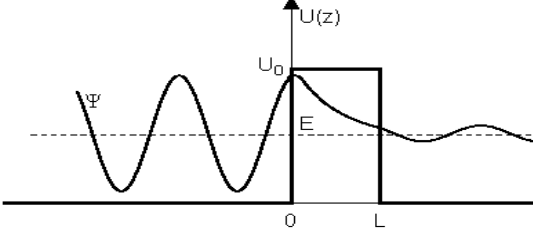
\includegraphics[width=3cm]{images/alpha_barrier.png} Barrier Penetration\\
$T = \frac{1}{1 + \frac{1}{4}\frac{U_{0}^{2}}{E(U_{0}-E)}sinh^{2}(\alpha L)}$\\
$\alpha = \sqrt{\frac{2m_{\alpha}E_{\alpha}}{\hbar^{2}}} \approx 17.5 fm$,  $T\approx10^{-29}$\\
BAD.  Instead, break up barrier into smaller chunks\\
$P \approx e^{-2\alpha a} = exp(-2\sqrt{\frac{2m_{\alpha}\frac{1}{2}(B-Q)}{\hbar^{2}}}x\frac{1}{2}(b-a))$\\
Coulomb barrier height (usually about 34 MeV for typical heavy nucleus):\\
$B = \frac{1}{4\pi \epsilon_{0}} \frac{zZ^{\prime}e^{2}}{a}$\\
Probability to penetrate the complete barrier is:\\
\hspace*{0.01\textwidth} $P = e^{-2G}$\\
$G = \sqrt{\frac{2m}{\hbar^{2}Q}}\frac{zZ^{\prime}e^{2}}{4\pi\epsilon_{0}}[arccos(\sqrt{x}) - \sqrt{x(1-x)}]$\\
Example: $\prescript{210}{}{Po} \rightarrow \prescript{206}{}{Pb} + \alpha$.  $E_{\alpha} = 5.4Mev$. Estimate height of coulomb barrier that $\alpha$ must tunnel through:  $r = \frac{1.25(210)^(1/3)}{2} = 3.714 fm$,\\ $B = \frac{e^{2}}{4\pi\epsilon_{0} \frac{(2)(82)}{3.714}} = 2(31.78)MeV?$\\
Estimate the probability that a 5.4MeV alpha particle in a head on collision wiht a $\prescript{206}{}{Pb}$ nucleus will penetrate the Coulomb barrier:  Use approx that $[arccos\sqrt{x} - \sqrt{x(x+1)}] \approx \frac{\pi}{2} - 2\sqrt{x}$ with $x = \frac{Q}{B}$.  Calc G then P.\\
Angular Momentum in Alpha Decay: Any angular momentum carried away by the $\alpha$-particle is purely orbital\\
Parity change = $(-1)^{\ell_{\alpha}}$.  If the initial and final parities are the same, $\ell$ is even.  If they are different, $\ell$ is odd.  For a given $\alpha$ energy Q, the probability of barrier penetration decreases with increasing $\ell$\\
Example: $\prescript{235}{}{U}$ decay:\\
 $\frac{\ell(\ell+1)}{2mr^{2}} = \frac{\ell(\ell+1)(197.3Mev f`m)^{2}}{2(4)(931.5Mev)(7.4fm)^{2}}$,\\ $\ell(\ell+1)x0.087Mev \rightarrow 0.174MeV$ for $\ell = 1$\\
 Alpha particle spectroscopy: 1. Make source of $\alpha$-decaying nuclei.  Must be thin for $\alpha$'s to escape without losing much energy.  2. Measure the number of $\alpha$'s as a function of their energies.  You can also measure g-rays emitted from excited states populated by $\alpha$ decay.\\

Copy hw 5 problems 8 and 10!!!\\

Beta Decay:\\
Neutrinos: No electric charge, interacts 'weakly' with matter (small xs), tiny mass, carries energy and linear momentum, has intrinsic spin of $\hbar /2$\\
$(Z,A) \rightarrow (Z-2,A-4) + \prescript{4}{}{He}_{2}$\\
$(Z,A) \rightarrow (Z\pm 1, A) + e^{\mp} + \nu_{e} (or) \bar{\nu_{e}}$\\
$\beta^{-}$ decay: \\
\hspace*{0.01\textwidth} $\prescript{210}{83}{Bi}_{127} \rightarrow \prescript{210}{84}{Ar}_{126} + e^{-} + \bar{\nu_{e}}$\\
\hspace*{0.01\textwidth} $(n\rightarrow p + e^{-} + \bar{\nu_{e}})$\\
$\beta^{+}$ decay: \\
\hspace*{0.01\textwidth} $\prescript{22}{11}{Na}_{11} \rightarrow \prescript{22}{10}{Ne}_{12} + e^{+} + \nu_{e}$\\
$B^{+}$ decay can occur if $Q_{ec} > 2m_{e}c^{2}$
\hspace*{0.01\textwidth} $(p\rightarrow n + e^{+} + \nu_{e})$\\
Electron Capture:\\
\hspace*{0.01\textwidth} $\prescript{22}{11}{Na}_{11} + e^{+} \rightarrow \prescript{22}{10}{Ne}_{12} + \nu_{e}$\\
\hspace*{0.01\textwidth} $(p + e^{-}\rightarrow n + \nu_{e})$\\
$Q_{\beta^{-}} = $\\$[M_{atomic}(\prescript{A}{Z}{X}_{N})-M_{atomic}(\prescript{A}{Z+1}{Y}_{N-1})]c^{2}$\\
$Q_{\beta^{-}} = T_{e} + T_{\bar{\nu}}$, since $T_{\bar{\nu}} \approx E_{\hat{\nu}}$\\
$T_{e}^{max} = E_{\bar{\nu}}^{max} = Q_{\beta^{-}}$\\
$Q_{\beta^{+}} = [M_{atomic}(\prescript{A}{Z}{X}_{N})$\\$ - M_{atomic}(\prescript{A}{Z-1}{Y}_{N+1}) + 2M_{e}]c^{2}$\\
EC-Decay: $\prescript{A}{Z}{X}_{N} + e^{-} \rightarrow \prescript{A}{Z-1}{Y}_{N+1} + \nu_{e}$\\
$Q_{ec} = [M_{atomic}\prescript{A}{Z}{X}_{N} $\\$ - M_{atomic}\prescript{A}{Z-1}{Y}_{N+1}]c^{2} - B_{n}$\\
$B_{n} = $ binding energy of captured $e^{-}$\\
Minimum Q value for $\beta^{+}$ decay: $Q_{\beta^{+}} > 2m_{e}c^2 = 1.022MeV$\\
Observed $Q_{\beta}$ values range from $\approx 2$keV to $\approx 20$ MeV. (Typical is around 1 MeV). 

Allowed Decays:\\
If electron and neutrino created at r = 0, they cannot carry any orbital angular momentum.  Change in angluar momentum of nucleus can only result from their spins.  If spins are antiparallel, it is a Fermi Decay (total S = 0, and $I_{i} = |I_{i} - I_{f}| = 0$).  If spins are parallel, called Gamow-Teller Decay, (total S = 1, and $I_{i} = I_{f} + 1)$.\\
Selection rules for allowed $\beta$ decay:\\
$\Delta I = 0,1$; $\Delta \pi$(parity change) = no\\
Ex:  Allowed $\beta$ decay: $\prescript{14}{}{O} \rightarrow \prescript{14}{}{N}^{*}$ ($0^{+} \rightarrow 0^{+}$).  Fermi Type.\\

Forbidden Decays (less probable):\\
First forbidden decays:$(l=1)$\\
\hspace*{0.01\textwidth} $\Delta I = 0,1,2$, $\Delta \pi = yes$\\
\hspace*{0.01\textwidth} Ex: $\prescript{17}{}{N} \rightarrow \prescript{17}{}{O}$, $(\frac{1}{2}^{-} \rightarrow \frac{5}{2}^{+})$\\
Second forbidden decays: $(l=2)$\\


\hspace*{0.01\textwidth} $\Delta I = 2,3$, $\Delta \pi = no$\\
\hspace*{0.01\textwidth} Ex: $\prescript{22}{}{Na} \rightarrow \prescript{22}{}{Ne}$, $(3^{+} \rightarrow 0^{+})$\\
Third forbidden decays: $(l=3)$ 
\hspace*{0.01\textwidth} $\Delta I = 3,4$, $\Delta \pi = yes$\\
\hspace*{0.01\textwidth} Ex: $\prescript{87}{}{Rb} \rightarrow \prescript{87}{}{Sr}$, $(\frac{3}{2}^{-} \rightarrow \frac{9}{2}^{+})$\\
Fourth forbidden decays: $(l=4)$
\hspace*{0.01\textwidth} $\Delta I = 4,5$, $\Delta \pi = no$\\
\hspace*{0.01\textwidth} Ex: $\prescript{115}{}{In} \rightarrow \prescript{115}{}{Sn}$, $(\frac{9}{2}^{+} \rightarrow \frac{1}{2}^{+})$\\

Cross section for reaction $\bar{\nu} + p \rightarrow n + e^{+}$ is $\sigma =$ probability per target atom for reaction / incident flux of $\bar{\nu}$

Helicity: All $\bar{\nu}$ have their spin vectors parallel to their momentum vectors, while all $\nu$ have spin opposite to momentum.  This property is called the helicity and is defined to be:\\
\hspace*{0.01\textwidth} $h = \frac{s \cdot p}{|s \cdot p|}$.  h $= 1$ for $\bar{\nu}$ and $-1$ for $\nu$\\
\hspace*{0.01\textwidth} Example: Using helicity of emitted $e^{-}$ and $\nu^{-}$, deduce whether the $e^{-}$ and $\nu^{-}$ tend to be emitted parallel or anti to one another: $\Delta L = 0$, so spin of emitted nuclei must be anti-parallel.  Helicity tells us that the momentum is aligned with this for the n and anti-aligned with this for the $e^{-}$ thus the particles tend to be emitted parallel to one another.  For $1^{+} \rightarrow 0^{+}$ $\beta^{-}$, using same logic but with $\Delta L = 1$, they tend to be emitted anti-parallel.\\

Gamma Decay:
E - electric, M - magnetic, dipole radiation.  Parity is:\\
\hspace*{0.01\textwidth} $\pi(ML) = (-1)^{L+1}$\\
\hspace*{0.01\textwidth} $\pi(EL) = (-1)^{L}$\\
Weisskopf Estimates:\\
\hspace*{0.01\textwidth} $\lambda (E1) = 1.0 \times 10^{14} A^{2/3} E^{3}$\\
\hspace*{0.01\textwidth} $\lambda (E2) = 7.3 \times 10^{7} A^{4/3} E^{5}$\\
\hspace*{0.01\textwidth} $\lambda (E3) = 34 A^{2} E^{7}$\\
\hspace*{0.01\textwidth} $\lambda (E4) = 1.1 \times 10^{-5} A^{8/3} E^{9}$\\
Note $\lambda$ is in $s^{-1}$ and E is in MeV\\
\hspace*{0.01\textwidth} $\lambda (M1) = 5.6 \times 10^{13} E^{3}$\\
\hspace*{0.01\textwidth} $\lambda (M2) = 3.5 \times 10^{7} A^{2/3} E^{5}$\\
\hspace*{0.01\textwidth} $\lambda (M3) = 16 A^{4/3} E^{7}$\\
\hspace*{0.01\textwidth} $\lambda (M4) = 4.5 \times 10^{-6} A^{2} E^{9}$\\

Angular momentum and parity selection rules:\\
$\Delta \pi = no$: even electric, odd magnetic\\
$\Delta \pi = yes$: odd electric, even magnetic\\

Example: List all permitted multipole modes and which is most likely (most intense) for $\frac{9}{2}^{-} \rightarrow \frac{7}{2}^{+}$.  $\Delta \pi = yes$, so $L = 1,2,3,4,5,6,7,$ or $8$.  $\Delta pi = $ yes, so Odd electric, even magnetic $ \rightarrow E1, M2, E3, M4, E5, M6, E7, M8$.  Most intense is E1.\\
$\lambda_{t} =$ total decay probability\\
$\lambda_{t} = \lambda_{\gamma} + \lambda_{e}$\\
$\alpha = \frac{\lambda_{e}}{\lambda_{\gamma}}$\\
$\lambda_{t} = \lambda_{\gamma}(1+\alpha)$\\
$\lambda_{t} = \lambda_{\gamma} + \lambda_{e,K} + \lambda_{e,L} + \lambda_{e,M} + ..$\\$ = \lambda_{\gamma}(1 + \alpha_{K} + \alpha_{L} + \alpha_{M} + ..)$\\
Nucleus Recoil: $T_{r} = \frac{E_{\gamma}^{2}}{2m_{r}c^{2}}$\\
Reaction Rate: $R = (\rho R)_{targ} \cdot I_{beam} \cdot \sigma_{rxn}$\\

Copy quarks and lepton stuff?\\
Copy forbidden decay problem from hw!!!!\\

Schrodingers Equation:\\
$-\frac{\hbar}{2m}\frac{d^{2}\psi}{dx^{2}} + V(x)\psi(x) = E\psi(x)$

Parity:  $|L| = \sqrt{l(l+1)}$\\

NEW STUFF (POST MT2):\\

PLAN:
In ne180 - know fission stuff.  Gives time to catch up\\
This week:  Read and go over with bernstein:\\
\hspace*{0.01\textwidth} chapter 4 (nuclear force)\\
\hspace*{0.01\textwidth} chapter 5 (nuclear structure)\\
\hspace*{0.01\textwidth} chapter 9\\
\hspace*{0.01\textwidth} Exam!!!!\\
Next week:  Read and go over with bernstein:\\
\hspace*{0.01\textwidth} chapter 10\\
\hspace*{0.01\textwidth} chapter 11\\
\hspace*{0.01\textwidth} chapter 12\\
Following week: decide accordingly\\

Chapter 4 (Nuclear Force):\\
Force between nucleons charge independent (acts on protons and neutrons)\\
Spins parallel, attractive, not, repulsive\\
Nuclear force tries to maximize itself.  Particles attempt to be as similar as possible, but still have to be different.  A proton and neutron will have parallel spins (difference is particle type) in a deuteron, while a proton and a proton system would have opposite spins.
GO OVER MAGNETIC DIPOLE MOMENTS\\
Classical: $\mu = \frac{e \hbar}{2 m} l $\\
QM: $\mu = g_{s}s\mu_{N}$\\
\hspace*{0.01\textwidth} $s$ is spin?\\
\hspace*{0.01\textwidth} $g_{s}$ is g factor
\hspace*{0.01\textwidth} $g_{s}^{proton} = 5.5856$\\
\hspace*{0.01\textwidth} $g_{s}^{neutron} = -3.82608$\\
\hspace*{0.01\textwidth} Not 0 for neutron, because neutron made up of charged particles (ddu,-1/3,-1/3,2/3), and they intrinsically spin.\\

Chapter 5 (Nuclear Models):\\

For the most part, I understand this chapter.  Go over understanding:

Shell Model: Works well with nuclei with A<20 as well as nuclei with magic numbers.\\
\hspace*{0.01\textwidth} EXPLAIN HOW TO DO SHELL POPULATION!!!!
\hspace*{0.01\textwidth} Gets better allowed energies and magic 
\hspace*{0.01\textwidth} numbers for higher A nuclei
\hspace*{0.01\textwidth} Shell model only good for nucleus with only one unpaired nuclei?  Different from extreme shell model because the single unpaired nuclei does not have to be the only nuclei in its level?\\
\hspace*{0.01\textwidth} Explain how to calculate magnetic dipole moments from shell model?

Go over Diagrams that show the shell model such as following:\\
\hspace*{0.01\textwidth} L13 Slide 2.  Numbers from closed shells\\
\hspace*{0.01\textwidth} Why do closed shells dramatically increase ionization energy?\\
\hspace*{0.01\textwidth} L13 Slide 4 - what is y axis?? \\
\hspace*{0.01\textwidth} L13 Slide 12 - explain please\\
\hspace*{0.01\textwidth} How well do we need to know rudimentary shell structure models that lead up to the final shell structure model introduced?\\
\hspace*{0.01\textwidth} This final shell model only works for odd A nuclei correct?
\hspace*{0.01\textwidth} Explain the Nilsson (deformed shell model), L13 S16 onward\

Work me through an example of finding the spin/parity for each model please?\\

$\mu = \mu_{N}(g_{l}l_{z} + g_{s}s_{z}) / \hbar$
Diagram on L14-16 Slide 8: linear increase for protons because $\mu \propto l$, no increase for neutrons because no charge!?\\
Electric Quadrupole Moment: Distribution of charge around nuclei.  Explain how to calculate from shell model?\\

Quiz me on it?\\

Extreme independent shell models:\\
Single particle nuclei (Independent Particle Model):\\
\hspace*{0.01\textwidth} 
Single hole nuclei (Independent particle model):\\
\hspace*{0.01\textwidth} All shells completely full/empty except for single missing nucleon in the highest energy filled shell\\
\hspace*{0.01\textwidth} Not same as shell model because in order to make single hole or particle condition, shells may be skipped/redistributed.  Correct?\\
Extreme independent model not the best because we can't attribute J to the last unpaired particle alone\\
Explain L14-16 Slide 15,16,why 17 is wrong, and 19/20!\\
Wtf is going on in L14-16 Slide 40\\
Explain L14-16 Slide 41\\

Quiz me on it?\\

Rotational Model:\\
Best for $150<A<190$ and $A>220$\\
$E \propto I^{2}$ where $I$ is angular momentum quantum number\\
Also, $E \propto \frac{1}{M_{I}}$ where MI is moment of inertia\\


Chapter 8 (alpha decay):\\

Go over and add questions for Wednesday.  I understand this chapter pretty well.\\

Chapter 9 (Beta decay):\\

Double Beta decay wtf\\
Takes place but implies neutrinos and antinuetrinos are not the same?  I thought the courier experiment proved that double beta decay could not happen?  L19-21 Slide 22\\

I think I understand beta decay pretty well\\
Go over diagrams in lecture:\\
\hspace*{0.01\textwidth}

Go over isomer states!\\
\hspace*{0.01\textwidth} What is a isomer\\
\hspace*{0.01\textwidth} Explain test problem!?\\

Future stuff to go over(not today):\\
Transfer of angular momentum in decays\\

Chapter??:

Nuclear Reactions:\\
Inelastic if Y or b is in an excited state\\
Need to know classifications for final? (p. 379)\\
$t1 =  (m_{Y}+m_{b})[m_{Y}Q + (m_{Y}-m_{a})T_{a}]$
$T_{b}^{1/2} = \frac{(m_{a}m_{b}T_{a})^{1/2}cos\theta \pm [ m_{a}m_{b}T_{a}cos^{2}\theta + t1 ]^{1/2}}{m_{Y} + m_{b}}$\\
Threshold value for $T_{a}$ for reaction:\\
\hspace*{0.01\textwidth} $T_{th} = (-Q)\frac{m_{Y} + m_{b}}{m_{Y}+m_{b}-m_{a}}$\\
What is the double-valued situation talked about on page 383?\\
Explain points 3 and 4 following this on page 384?\\
Isospin:\\
\hspace*{0.01\textwidth} Proton: isospin-up. $m_{t} = \frac{1}{2}$\\
\hspace*{0.01\textwidth} Neutron: isospin-down $m_{t} = -\frac{1}{2}$\\
\hspace*{0.01\textwidth} t length = $\sqrt{t(t+1)}\hbar$\\
\hspace*{0.01\textwidth} 3 axis projection $t_{3} = m_{t}\hbar$\\
\hspace*{0.01\textwidth} $T_{3} = \frac{1}{2} (Z-N)$\\
\hspace*{0.01\textwidth} Total isospin must be at least $T_{3}$\\
I don't understand spin units (all units of hbar).  Explain?\\
Explain solid angle again?? Just fraction of surface area?\\

Reaction Cross Sections:\\
$\sigma \frac{R_{b}}{I_{a}N}$, Outgoing particles of rate $R_{b}$\\
Differential xs: $\frac{d\sigma}{d\Omega} = \frac{r(\theta,\phi)}{4\pi I_{a} N}$\\
To what extent do we have to know the differentials for cross section?  There are a lot of them!\\


Nuclear Fission (Chapter 13):\\

Fission products not symmetric because of coulomb barrier.  Ie, $\prescript{235}{}{U}$ can exist as two $\prescript{119}{}{Pd}$ nuclei, but they cannot separate due to the enormous coulomb barrier.  Different sizes reduces the coulomb barrier, making fission more likely.\\
Height of coulomb barrier is roughly equal to the energy released in fission of heavy nuclei\\
Spontaneously fissioning nuclei have energy release that puts the two fragments just below the Coulomb barrier, giving them a reasonably good chance to penetrate.  Explain??  Page 481\\
$\beta$ delayed neutrons are a result of $\beta$ decay of the fission products\\
Excitation Energy:\\
\hspace*{0.01\textwidth} $E_{ex} = [m(\prescript{236}{}{U}^{*}) - m(\prescript{236}{}{U})]$, $m(\prescript{236}{}{U}^{*}) = m(\prescript{235}{}{U}) + m_{n}$ for$\prescript{235}{}{U}$ neutron capture\\

If activation energy less than excitation energy, fission results.  In this case, it does!\\


Things I have trouble with/should spend more time on:\\
\hspace*{0.01\textwidth} Connecting what we learn in terms of equations and concepts with nuclear diagrams/graphs/plots\\
\hspace*{0.01\textwidth} Understanding 


Nuclear Fusion (Chapter 14):\\

Energy Release:\\
$\frac{1}{2}m_{b}v_{b}^{2} + \frac{1}{2}m_{Y}v_{Y}^{2} \approx Q$\\
$\frac{1}{2}m_{b}v_{b}^{2} \approx \frac{Q}{1 + m_{b}/m_{Y}}$\\
$\frac{1}{2}m_{Y}v_{Y}^{2} \approx \frac{Q}{1 + m_{Y}/m_{b}}$\\

Coulomb Barrier:\\
$V_{c} = \frac{e^{2}}{4\pi \epsilon_{0}}\frac{Z_{a}Z_{X}}{R_{a}+R_{X}}$\\

Cross Section:\\
$\sigma \propto \frac{1}{v^{2}} e^{-2G}$\\
$G = \frac{e^{2}}{4\pi \epsilon_{0}}\frac{\pi Z_{A} Z_{X}}{\hbar v}$, $v$ is relative velocity\\

LOTS OF OTHER STUFFFFFF\\

Detectors (Chapter 7):\\


ADD CYLINDRICAL COORDINATES AND JACOBIAN!\\
$r = \rho?$, theta vertical angle\\
$x = \rho sin\theta cos\phi$\\
$y = \rho sin\theta sin\phi$\\
$z = \rho cos\theta$\\
$dxdydz = \rho^{2}sin\theta d\rho d\theta d\phi$\\
blank\\
blank\\
blank\\
blank\\
blank\\
blank\\
blank\\
blank\\
blank\\
blank\\
blank\\
blank\\
blank\\
blank\\
blank\\
blank\\
blank\\
blank\\
blank\\
blank\\
blank\\
blank\\
blank\\
blank\\
blank\\
blank\\
blank\\
blank\\
blank\\
blank\\
blank\\
blank\\
blank\\
blank\\
blank\\
blank\\
blank\\
blank\\
blank\\
blank\\
blank\\
blank\\
blank\\
blank\\
blank\\
blank\\
blank\\
blank\\
blank\\
blank\\
blank\\
blank\\
blank\\
blank\\
blank\\
blank\\
blank\\
blank\\
blank\\
blank\\
blank\\
blank\\
blank\\
blank\\
blank\\
blank\\
blank\\
blank\\
blank\\
blank\\
blank\\
blank\\
blank\\
blank\\
blank\\
blank\\
blank\\
blank\\
blank\\
blank\\
blank\\

\end{multicols}
 
\end{document}